\documentclass[10pt,twocolumn]{article}
\usepackage{geometry}
\geometry{verbose,headsep=3cm,tmargin=2.5cm,bmargin=2.5cm,lmargin=2.0cm,rmargin=2.0cm}
\usepackage{graphicx}
\usepackage{xcolor}
\usepackage[font=small]{caption}
\usepackage{amsmath,amssymb,latexsym}
\usepackage{marvosym}
\usepackage{url}
\usepackage{lipsum}
\usepackage{bm}
\usepackage{float}
\usepackage[english]{babel}
\usepackage{hyperref}
\usepackage{epsf}
\usepackage{float}
\usepackage{mathpazo}
\usepackage{pifont}
\usepackage{wrapfig}
\usepackage{multicol}
\usepackage{enumitem}
\usepackage{xcolor}
\usepackage{framed}
\usepackage[utf8]{inputenc}
% Document font:
\usepackage{charter}
\graphicspath{{DWGs/}}

\begin{document}

\twocolumn[{
\begin{@twocolumnfalse}

  \begin{center}
%\textcolor{lgray}
    \vskip-5em

    \hfill
    \fontsize{10}{10}\selectfont {\textit{Bruxelles, August 2019}}

    \vskip2ex
    
	\vspace{5ex}
	
    \fontsize{24}{10}\selectfont {Chemical source term regression}
    



  \noindent%
    
\vskip1ex

{\rule{\textwidth}{0.5pt}}

  \end{center}
  
    \fontsize{7}{10}\selectfont {This work is licensed under the Creative Commons Attribution-NonCommercial-ShareAlike 4.0 International (CC BY-NC-SA 4.0) license.}

\vspace{6mm}

\end{@twocolumnfalse}
}]

\setlength{\parindent}{0cm}

\vspace{10mm}

\setlength{\parindent}{0cm}

\fontsize{14}{10}\selectfont {Kamila Zdybał}

\vspace{2mm}

\fontsize{8}{10}\selectfont {\textit{Université libre de Bruxelles, kamila.zdybal@ulb.ac.be}}

\fontsize{8}{10}\selectfont {\textit{camillejr.github.io/science-docs, kamila.zdybal@gmail.com}}

\vspace{2mm}



\section*{Preface}

State of my knowledge on chemical source terms.

\,\,

This document is still in preparation. Please feel free to contact me with any suggestions, corrections or comments.

\section*{Keywords}

\textit{Principal Component Analysis, chemical source}



\tableofcontents


\section{The chemical source}




\section{PC-sources}

The original chemical sources are linearly transformed using the matrix $\mathbf{A}$ of Principal Component modes and each PC-source term is additionally scaled by the corresponding scaling factor stored in a vector $\mathbf{d}$.

\begin{equation}
\mathbf{S_z} = \mathbf{S} \mathbf{A} \cdot \mathbf{d}^{-1}
\end{equation}

Each PC-source is a linear combination of the original sources (columns of $\mathbf{S}$). Each PC-source is computed from only one Principal Component (column of $\mathbf{A}$).

\begin{figure}[H]
\centering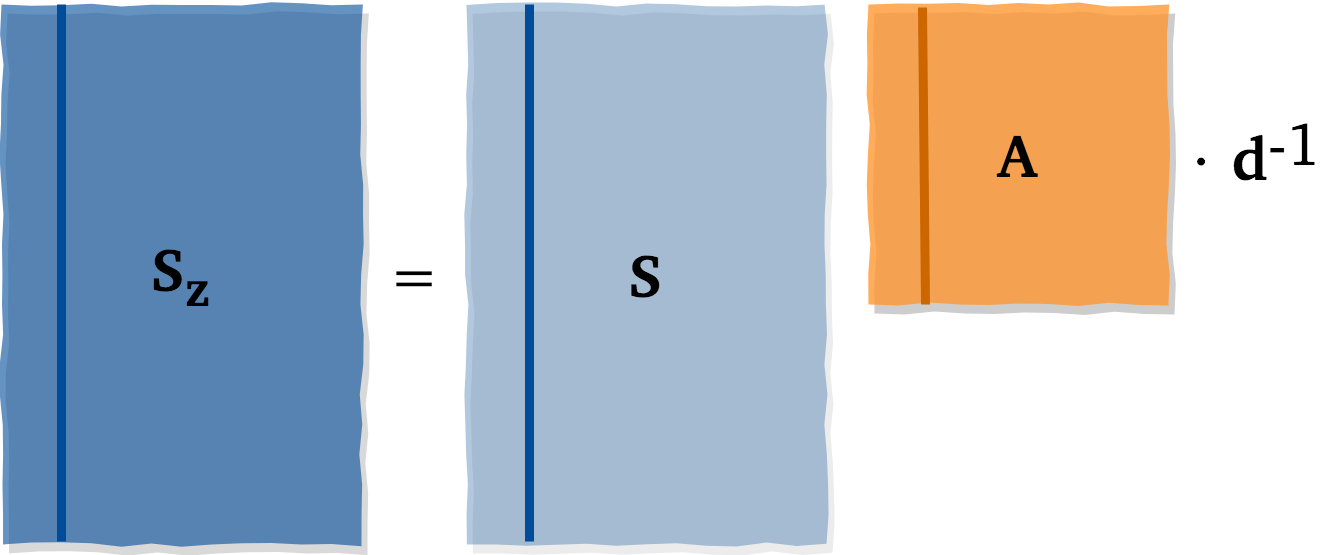
\includegraphics[width=7cm]{PC-source-computation.png}
\caption{Computation of the PC-sources (columns of $\mathbf{S_z}$).}
\label{fig:PC-source-computation}
\end{figure}



\thebibliography{}

\bibitem{}
\end{document}
